%----------------------------------------------------------------------------------------
% Biobank V4 Design
%
% The latest version of this document is kept on GitHub at:
%
% https://github.com/cbsrbiobank/biobankv4design
%
% Command to a PDF document:
%
%   > rubber --pdf main
%----------------------------------------------------------------------------------------

\documentclass[10pt,twoside,letterpaper]{memoir}
% Page margins
\usepackage[top=3cm,bottom=3cm,left=3.2cm,right=3.2cm,headsep=10pt,a4paper]{geometry}

\usepackage{bookman} % font used for text
\usepackage[T1]{fontenc}
\usepackage{titlesec} % Allows customization of titles

\usepackage{tabularx,environ}

\usepackage[english]{babel} % English language/hyphenation
\usepackage{booktabs} % Required for nicer horizontal rules in tables
\usepackage{graphicx} % Required for including pictures

\usepackage[svgnames]{xcolor} % Required to specify font colors

\usepackage[utf8]{inputenc} % Required for including letters with accents
\usepackage{csquotes}

\usepackage{microtype} % Slightly tweak font spacing for aesthetics
\usepackage{enumitem} % allows lists to be customized
\usepackage{float} % figure placement

% the float package disables table repositioning
\usepackage{float}
\restylefloat{table}

\DeclareMathAlphabet{\mathpzc}{OT1}{pzc}{m}{it}
\DeclareGraphicsExtensions{.pdf,.png,.jpg}

%----------------------------------------------------------------------------------------
% Colors used in document
%----------------------------------------------------------------------------------------

\definecolor{Blue}{rgb}{.204,.353,.541}
\definecolor{DarkBlue}{RGB}{46,71,108}
\definecolor{LightBlue}{RGB}{76,129,188}
\definecolor{Green}{RGB}{155,186,87}
\definecolor{DarkGreen}{RGB}{86,114,44}
\definecolor{Orange}{RGB}{248,150,71}
\definecolor{DarkOrange}{RGB}{187,115,53}
\definecolor{Purple}{RGB}{129,99,162}
\definecolor{DarkPurple}{RGB}{94,72,120}
\definecolor{gray75}{gray}{0.75}

%----------------------------------------------------------------------------------------
% PDF settings
%----------------------------------------------------------------------------------------

\usepackage[pdftex,
  pdfauthor={AICML},
  pdftitle={BioBank V4 Design},
  colorlinks,
  linktoc=all,
  linkcolor=Blue,
  urlcolor=Purple,
  citecolor=Blue,
  bookmarks=true,
  bookmarksopen=true,
  pdfstartview=FitH]
	   {hyperref}

\hypersetup{
}

%----------------------------------------------------------------------------------------
% Bibliography settings
%----------------------------------------------------------------------------------------

\usepackage[
  style=alphabetic,
  sorting=nyt,
  sortcites=true,
  autopunct=true,
  babel=hyphen,
  hyperref=true,
  abbreviate=false,
  backref=true,
  backend=biber
]{biblatex}
\addbibresource{bibliography.bib} % BibTeX bibliography file
\defbibheading{bibempty}{}

%----------------------------------------------------------------------------------------
% Chapter and section formating - using 'ell' chapter style with customizations
%----------------------------------------------------------------------------------------

\chapterstyle{ell}
\renewcommand*{\chapnumfont}{\normalfont\Huge\bfseries\sffamily\color{Blue}}
\renewcommand*{\chaptitlefont}{\normalfont\Huge\bfseries\sffamily\color{Blue}}
\renewcommand*{\secheadstyle}{\normalfont\Large\bfseries\sffamily\color{Blue}}
\renewcommand*{\subsecheadstyle}{\normalfont\normalsize\bfseries\sffamily\color{LightBlue}}

\setcounter{secnumdepth}{3}
\setsecnumdepth{subsection}

%----------------------------------------------------------------------------------------
%	TITLE PAGE
%----------------------------------------------------------------------------------------

\newcommand*{\titleTH}{\begingroup % Create the command for including the title page in the document
\raggedleft % Right-align all text
\vspace*{\baselineskip} % Whitespace at the top of the page

% Author % name
{\Large\bfseries\sffamily Author: Nelson Loyola}\\[0.167\textheight]

{\hfill\rule{.7\textwidth}{2pt}}\vspace*{\baselineskip}

% First part of the title
{\LARGE\bfseries\sffamily Biobank V4}\\[\baselineskip]

% Main title which draws the focus of the reader
{\textcolor{Blue}{\Huge\bfseries\sffamily Design Document}}\\[\baselineskip]

{\large\bfseries\sffamily \textit{Draft 0.1}}

{\hfill\rule{.7\textwidth}{2pt}}

% Whitespace between the title block and the publisher
\vfill

% Publisher and logo
{\large\bfseries\sffamily
  \href{http://biosample.ca/}{Prepared for the Canadian Biosample Repository} \\
  by the \href{http://www.aicml.ca/}{Alberta Innovates Center for Mathine Learning}\\ }\par
\vspace*{\baselineskip}
{\textcolor{Blue}{
    \small\sffamily University of Alberta\\
    Department of Computing Science\\
    2-21 Athabasca Hall\\
    Edmonton, Alberta\\
    \href{mailto:info@aicml.ca}{info@aicml.ca}
}}

\vspace*{3\baselineskip} % Whitespace at the bottom of the page
\endgroup}

%----------------------------------------------------------------------------------------
% Table of contents
%----------------------------------------------------------------------------------------

\usepackage[textsize=small, backgroundcolor=Orange, bordercolor=Orange, shadow]{todonotes}

\renewcommand{\cftchapterfont}{\normalfont\bfseries\sffamily}
\renewcommand{\cftsectionfont}{\normalfont\sffamily}
\renewcommand{\cftsubsectionfont}{\normalfont\sffamily}
\renewcommand{\cftchapterpagefont}{\normalfont\sffamily\bfseries}
\renewcommand{\cftsectionpagefont}{\normalfont\sffamily}
\renewcommand{\cftsubsectionpagefont}{\normalfont\sffamily}

\maxtocdepth{subsection}

\AtBeginDocument{\renewcommand\contentsname{Table of Contents}}

%----------------------------------------------------------------------------------------
% hyperlinks to entities and value objects
%----------------------------------------------------------------------------------------

\newcommand{\entitytarget}[1]{\hypertarget{#1}{\texttt{\textbf{\color{Blue}#1}}}}
\newcommand{\valobjtarget}[1]{\hypertarget{#1}{\texttt{\textbf{\color{Blue}#1}}}}

\newcommand{\entitylink}[1]{\hyperlink{#1}{\texttt{\textbf{#1}}}}
\newcommand{\valobjlink}[1]{\hyperlink{#1}{\texttt{\textbf{#1}}}}

%----------------------------------------------------------------------------------------
% environment to help with command arguments tables
%
% the first column is the argument name, second is the java type, and third is
% the a description.
%----------------------------------------------------------------------------------------

\NewEnviron{commandparmtable}{%
  \begin{table}[H]
  \renewcommand{\arraystretch}{1.2}
  \small
  \begin{tabularx}{\textwidth}{l l X}
  \sffamily{\textbf{Parameter}} & \sffamily{\textbf{Type}} & \sffamily{\textbf{Description}} \\ \hline
  \BODY
  \hline
  \end{tabularx}
  \end{table}
}

%----------------------------------------------------------------------------------------
% macros
%----------------------------------------------------------------------------------------

\newcommand{\compfont}[1] {\texttt{\textbf{#1}}}

%----------------------------------------------------------------------------------------
% Document start
%----------------------------------------------------------------------------------------

\begin{document}
\frontmatter

\thispagestyle{empty} % Removes page numbers
\titleTH % This command includes the title page

\clearpage
\tableofcontents
\clearpage
%\listoffigures
%\clearpage
%\listoftodos
%\clearpage

\mainmatter
\chapter{Introduction}

Biobank version 4 is a rewrite of the Biobank application, meant to provide the
majority of its functionality through a web browser based interface. It was
designed using Domain Driven Design principles \cite{evans2004domain} and
employs a CQRS architecture (Command Query Responsibility Segregation)
\cite{vernon2013implementing}.

In addition, version 4 includes enhancements to the domain model which provides
better workflow and an improved user experience.

Flatbed scanning is supported by having a separate dedicated client, but this
client's functionality is focused only on scanning and decoding tubes etched
with 2D barcodes.

\section{Dependencies}

This version of Biobank uses the following open source tools / software packages:

% table with no indentation
\begin{description}

  \item[Jetty Http Server] \hfill \\ The Embedded Jetty Server provides web
    browser with access to the application.

  \item[MongoDB ] \hfill \\ A document based NoSQL database and provides an
    event store implementation that stores event streams in a MongoDB database.

  \item[MySQL database ] \hfill \\ A SQL relational database management sytem
    used to store the query model.

  \item[Axon Framework ] \hfill \\ Provides the building blocks used in
    applying the CQRS architectural pattern.

  \item[Spring Framework ] \hfill \\ Provides a comprehensive programming and
    configuration model for modern Java-based enterprise applications.

  \item[Spring MVC ] \hfill \\ Model-view-controller framework for web
    applications.

  \item[Spring Security ] \hfill \\ A customizable authentication and
    access-control framework for securing web applications.

  \item[Hibernate ] \hfill \\ An object-relational mapping library that
    provides a framework to map a data model to a relational database.

  \item[Twitter Bootstrap ] \hfill \\ Bootstrap is a sleek, intuitive, and
    powerful front-end framework for faster and easier web user interface
    development \cite{bootstrap}

\end{description}

\section{CQRS}

There are a number of reasons for choosing the CQRS architecture for
Biobank. Amongst these are:

\begin{itemize}
\item Employs a message-based system that allows for decoupling and is more
  reliable against transient failures.
\item \textbf{Commands} (that change data) are separated from \textbf{queries}
  (that read data).
\item Enables domain driven design by capturing the intent in the form of
commands.
\item \textbf{Event Sourcing} allows persisting of application entities as a
  sequence of events that created them. Thus, captures all business changes in a
  lossless manner.
\item Events are used to populate views also known as the reporting side. Thus,
  allows for decoupling of domain logic from reporting.
\item Allows for definitions of new reports that provide new insight to the
  data that has already been captured.
\end{itemize}

\chapter{Architecture}

\section{External Architecture}

The Biobank application uses a hexagonal architecture to interface to internal
and external clients, external services, and for data storage. Figure
\ref{fig:hex-architecture} shows the how the ports are configured. Web browser
based clients access the application via the internal client port. A RESTful
interface is also supported to allow the Biobank scanning client access via the
external client port. External systems can also access the application via this
port. Biobank can communicate to external services by using the external
services port. The figure also shows that the event store and query databases
are accessed via dedicated ports.

\begin{figure}[h]
  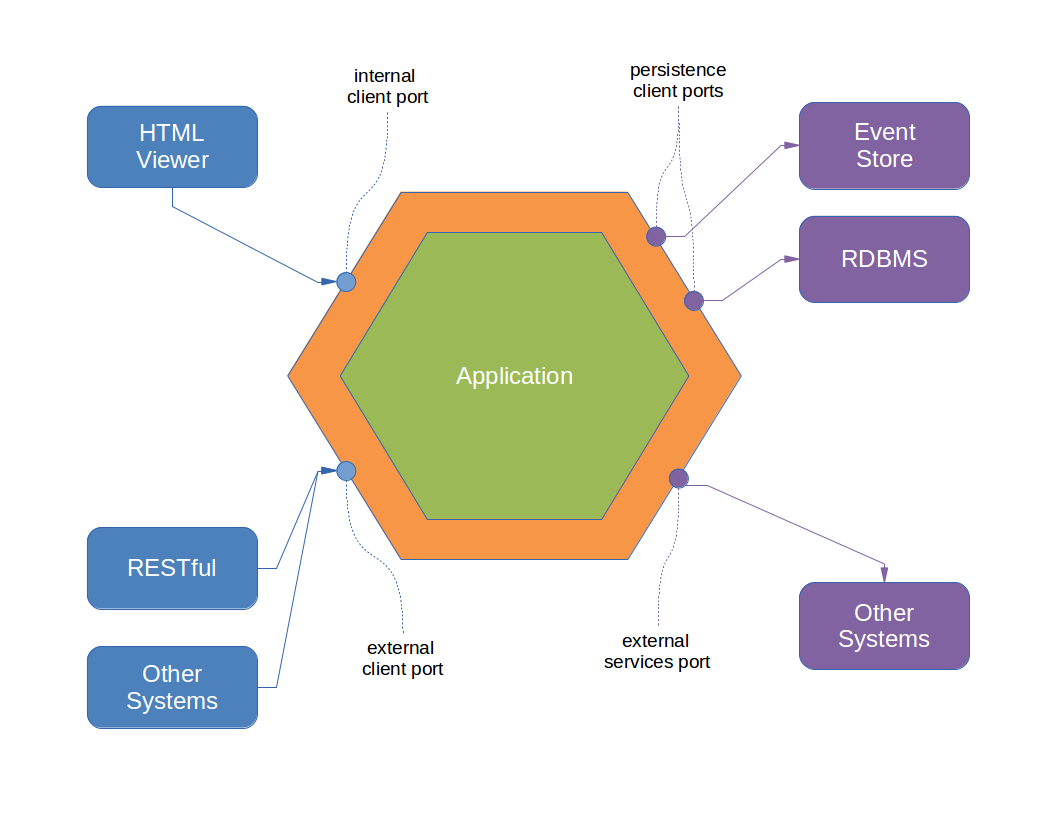
\includegraphics[trim={15mm 18mm 15mm 12mm}, clip, width=1\textwidth]{images/hex-architecture}
  \caption{Hexagonal architecture}
  \label{fig:hex-architecture}
\end{figure}

\section{Interal Architecture}

The client ports shown in Figure \ref{fig:hex-architecture} are managed by
client adapters. These client adapters then interface to the rest of the system
via the \emph{Command Bus} and the \emph{Query Interface} provided by the
\emph{Thin Data Layer}. Figure \ref{fig:cqrs-architecture} shows a more detailed
view of the application. It is the architecture recommended by the Axon
Framework\footnote{The figure and the material that follows is borrowed from
  the Axon Framework Reference Guide \cite{AxonOnline}}.

\begin{figure}[h]
  \begin{center}
    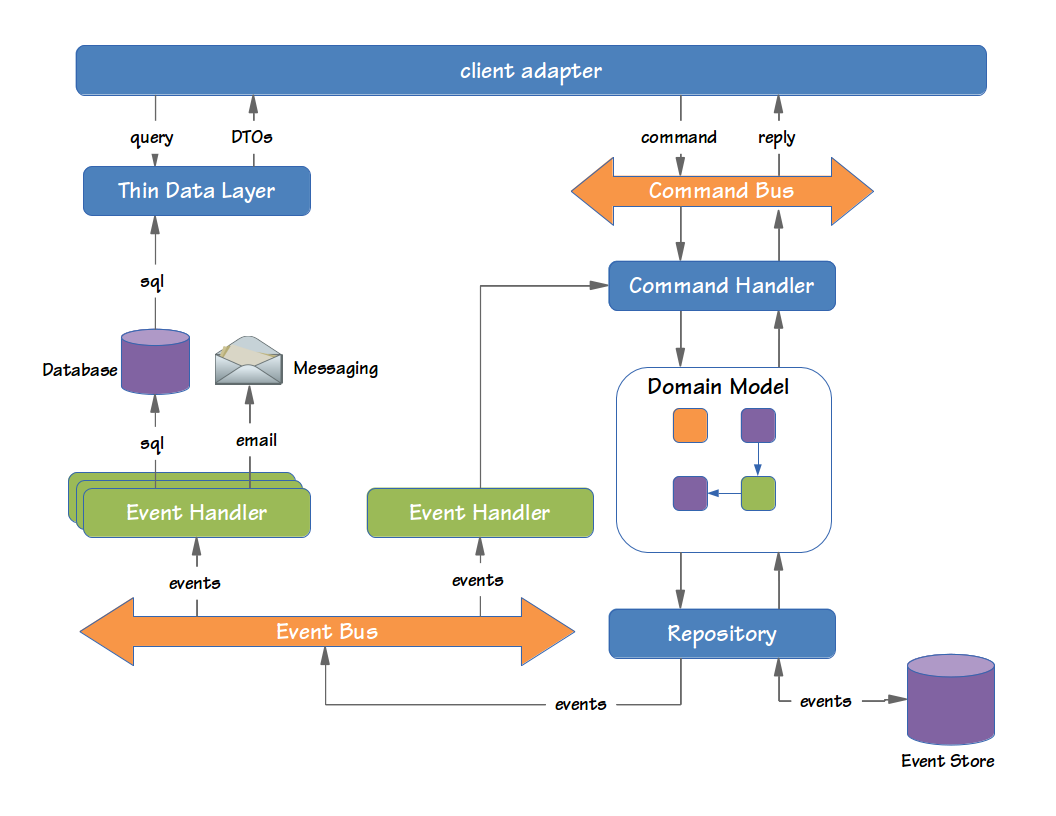
\includegraphics[trim={10mm 5mm 15mm 10mm}, clip, width=1\textwidth]{images/cqrs-architecture}
    \caption{Biobank architecture}
    \label{fig:cqrs-architecture}
  \end{center}
\end{figure}

\section*{Command Handling}

Commands are typically represented by simple and straightforward objects that
contain all data necessary for a command handler to execute it. A command
expresses its intent by its name. In Java terms, that means the class name is
used to figure out what needs to be done, and the fields of the command provide
the information required to do it.

The Command Bus receives commands and routes them to the Command Handlers. Each
command handler responds to a specific type of command and executes logic based
on the contents of the command. In some cases, however, logic is executed
regardless of the actual type of command, such as validation, logging or
authorization.

\section*{Domain Model}

The command handler retrieves domain objects (Aggregates) from a repository and
executes methods on them to change their state. These aggregates typically
contain the actual business logic and are responsible for guarding their own
invariants. The state changes of aggregates result in the generation of Domain
Events. Both the Domain Events and the Aggregates form the domain model.

\section*{Repositories and Event Stores}

Repositories are responsible for providing access to aggregates. Typically,
these repositories are optimized for lookup of an aggregate by its unique
identity. Repositories store the state changes that the aggregate has gone
through in an Event Store. The repository is also responsible for persisting
the changes made to aggregates in its backing storage.

\section*{Event Processing}

The event bus dispatches events to all interested event handlers. This is done
synchronously or asynchronously. Asynchronous event dispatching allows the
command execution to return and hand over control to the user, while the events
are being dispatched and processed in the background. Not having to wait for
event processing to complete makes an application more responsive. Synchronous
event processing, on the other hand, is simpler and is a sensible
default. Synchronous processing also allows several event listeners to process
events within the same transaction.

Event handlers receive events from the event bus. Some handlers update data
sources used for querying while others send messages to external
systems. Command handlers are completely unaware of the components that are
interested in the changes they make. This means that it is very non-intrusive
to extend the application with new functionality. All you need to do is add
another event handler. The events loosely couple all components in your
application together.

In some cases, event processing requires new commands to be sent to the
application. The saga is the CQRS concept responsible for managing these
complex business transactions.

\section*{Querying for data}

The thin data layer in between the client adapters and the data sources
provides a clearly defined interface to the actual query implementation
used. This data layer typically returns read-only Data Transfer Objects (DTOs)
containing query results. The contents of these DTOs are typically driven by
the needs of the client adapters. In most cases, they map directly to a
specific view in the UI (also referred to as table-per-view).

\subsection{Axon Framework Modules}

The Axon Framework provides a number of different modules that target specific
problem areas of CQRS. This section describes which modules were chosen.

\todo[inline]{This section is incomplete.}

\chapter{Domain Model}

The Biobank application is composed different modules\footnote{The term ``Module''
  is used in the context described in \cite{vernon2013implementing}}. Each
module is described briefly here and in more details are provided in the
remaining chapters.


\begin{description}

  \item[Study Configuration] \hfill \\

  \item[Patient Collection] \hfill \\

  \item[Specimen Processing] \hfill \\

  \item[Center Shipment] \hfill \\

  \item[Center Configuration] \hfill \\

  \item[Center Storage Configuration] \hfill \\

  \item[Specimen Request] \hfill \\

\end{description}

\chapter{Study Management}
\label{chap:study-management}

This section first describes the study aggregate, its composition, and then
defines the commands it handles.

The \entitytarget{Study} aggregate is used to configure different aspects for a
study. It is used to define the valid types of specimens that can be collected
from participants, when they are to be collected, how the collected specimens
are processed, and allows for customization with use of annotation types. This
aggregate is made up of the entities and value objects shown in the figure
below.

\begin{figure}[H]
  \centering
  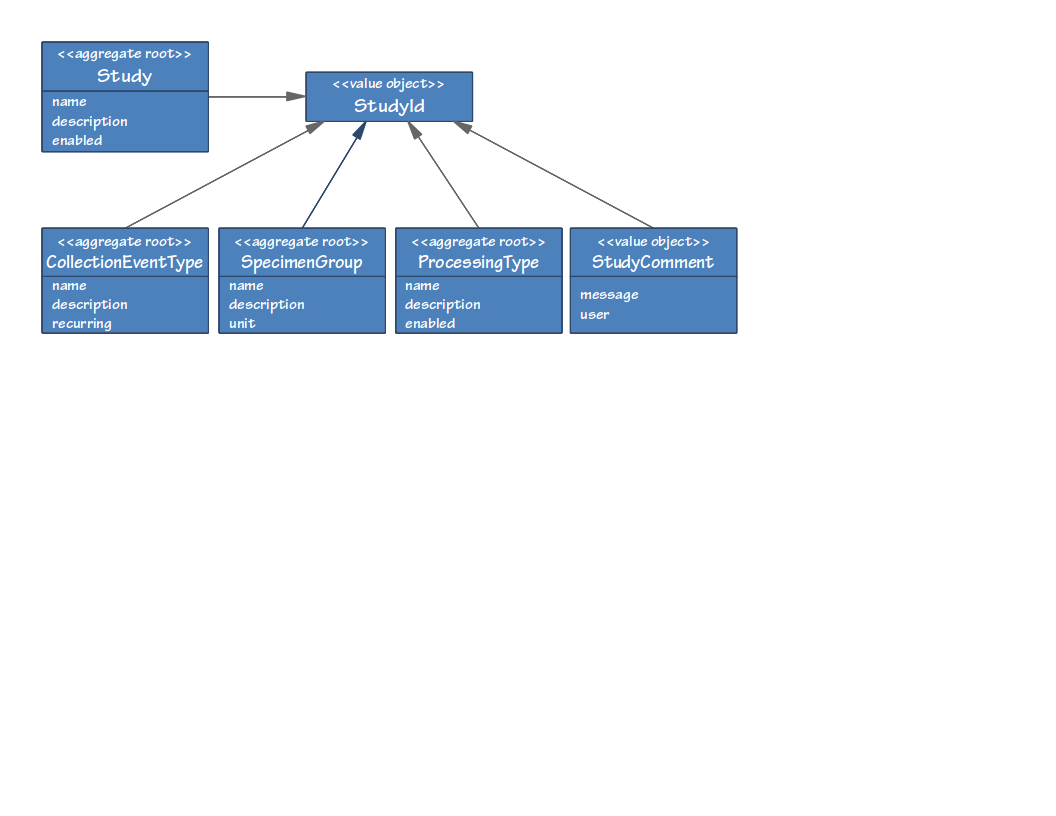
\includegraphics[trim={9mm 76mm 36mm 18mm}, clip,
    width=1\textwidth]{images/study-aggregate}
  \caption{Study aggregate}
  \label{fig:study-aggregate}
\end{figure}

\subsection*{Study}

A \entitylink{Study} represents a collection of participants and specimens
collected for a particular research study. Each study has a unique identifier,
\compfont{StudyId}, that is used to reference it. The \compfont{name} is a short
descriptive name, unique within the application, that is usually an acronym
used for quick identification.  The \compfont{description} give more details on
the name and is usually the words that make up the acronym.

A study can be enabled or disabled. When disabled, changes to its configuration
are possible but patients and specimens cannot be added. When enabled, no
further configuration changes are allowed, and participants and specimens can
be added.

As shown in the Figure \ref{fig:study-aggregate}, the study has collections of
other entities and value objects which are described below.

\subsection*{SpecimenGroup}

A \entitytarget{SpecimenGroup} is used to configure a specimen type used by the
study.  It records ownership, summary, storage, and classification information
that applies to an entire group or collection of \entitylink{Specimen}s. A
specimen group is defined either for specimens types collected from
participants, or for specimen types that are processed. More details for this
entity are given in Section \ref{sec:specimen-group}.

\subsection*{CollectionEventType}
A \entitytarget{CollectionEventType} defines a classification name, unique to
the \entitylink{Study}, to a participant visit. A participant visit is a record
of when specimens were collected from a participant at a collection
centre. Each collection event type is assigned one or more specimen groups to
specify the specimen types that are collected. See Section
\ref{sec:collection-event-type} for more details.

\subsection*{ProcessingType}
A \entitytarget{ProcessingType} describes a regularly performed specimen
processing procedure with a unique name (unique to the
\entitylink{Study}). There should be one or more associated
\entitylink{SpecimenLinkType}s that (1) further define legal procedures and (2)
allow recording of procedures performed on different types of
\entitylink{Specimen}s. See Section \ref{sec:processing-type} for more details.

\subsection*{StudyAnnotationType}

\entitytarget{StudyAnnotationType}s allows a study to collect custom named and
defined pieces of data on collection event types (Section
\ref{sec:collection-event-type}), processing events (Section
\ref{sec:processing-type}), and participants (Section
\ref{chap:study-annotations}). Annotations are optional and are not a
requirement for specimen collection or processing.

\subsection*{StudyComment}
A \entitytarget{StudyComment} contains a textual message and the user that
added the comment. The date and time the comment is made is recorded as meta
data. A study can have one or more comments.

\section{SpecimenGroup Details}
\label{sec:specimen-group}

The \entitylink{SpecimenGroup} entity is composed of the value objects shown
in Figure \ref{fig:specimen-group}.

A specimen group has a name and an optional description. The name is a short
identifying name that is unique to the study, and the description can provide
additional details on the name. The unit specifies how the specimen amount is
measured (e.g. volume, weight, length, etc.).

A study can have one or more specimen groups. For specimen collection to be
allowed on a study, at least one specimen group must be defined.

\begin{figure}[H]
  \centering
  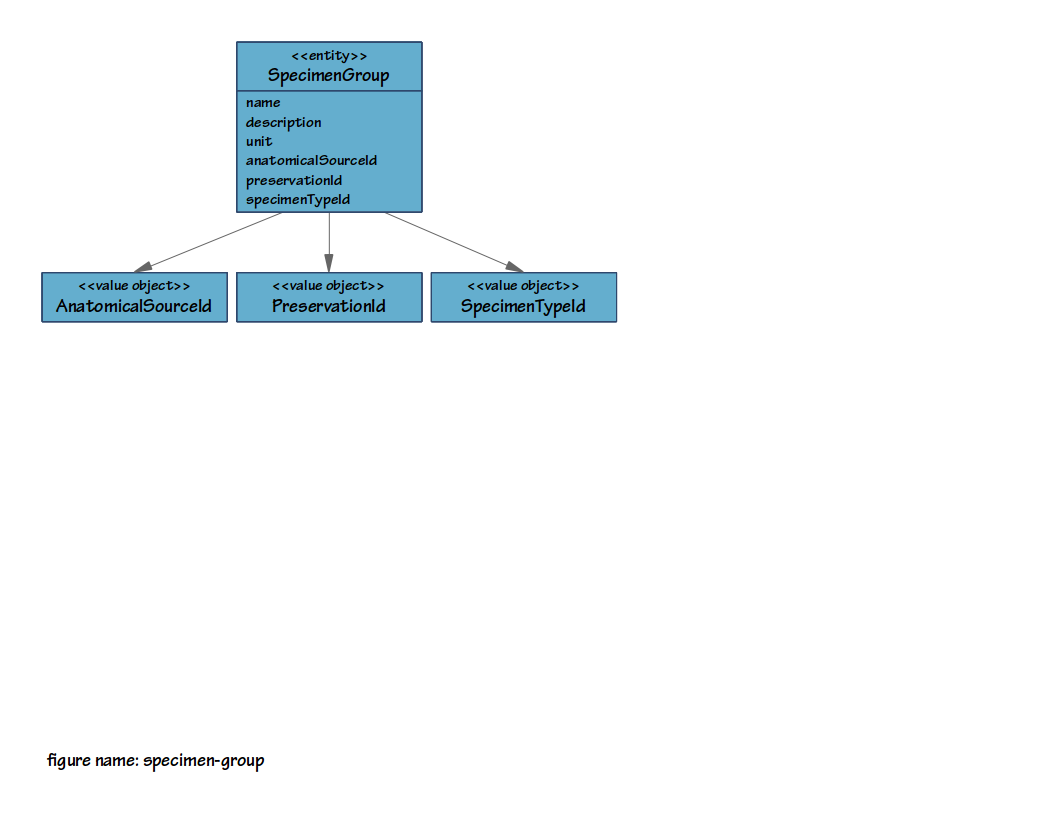
\includegraphics[trim={9mm 120mm 80mm 18mm}, clip,
    width=1\textwidth]{images/specimen-group}
  \caption{SpecimenGroup entity}
  \label{fig:specimen-group}
\end{figure}

\subsection*{AnatomicalSourceId}

An \valobjlink{AnatomicalSource} is a standardized set of regions from a
\entitylink{Participant} \emph{where} a \entitylink{Specimen} is collected
from. Potential examples include: colon, ear, leg, kidney,
etc. \valobjlink{AnatomicalSource} is a value object with a unique ID. They are
defined globally and new ones can be created at any time. They can be accessed
via look up service described in Section \ref{sec:lookup-service}.

A specimen group contains the ID of a single anatomical source.

\subsection*{PreservationId}

\valobjlink{Preservation} is a value object that describes how a
\entitylink{Specimen} should be preserved/stored by describing temperature
requirements ($^\circ$C), as well as a preservation method (see
\valobjlink{PreservationType}). \valobjlink{Preservation} is also a value
object with a unique ID. They are defined globally and new ones can be created
at any time. They can be accessed via look up service described in Section
\ref{sec:lookup-service}.

A specimen group contains the ID of a single preservation object.

\subsection*{SpecimenTypeId}

\valobjlink{SpecimenType} is standardized set of classifications that describe
\emph{what} a \entitylink{Specimen} is. Potential examples include: urine,
whole blood, plasma, nail, protein, etc. \valobjlink{SpecimenType} is also a
value object with a unique ID. They are defined globally and new ones can be
created at any time. They can be accessed via look up service described in
Section \ref{sec:lookup-service}.

A specimen group contains the ID of a single specimen type.

\section{CollectionEventType Details}
\label{sec:collection-event-type}
A collection event type has a name and an optional description. The name is a
short identifying name that is unique to the study, and the description can
provide additional details on the name. The \compfont{recurring} field is set to
\compfont{true} when the collection event type occurs more than once during the
lifetime of the study.

A collection event type can be configured to collect one or more specimens using
\entitylink{SpecimenGroupCollectionEventType}. It can also be configured to
record one or more annotation types using
\entitylink{CollectionEventTypeAnnotationType}. These associations are shown in
Figure \ref{fig:collection-event-type}.

A study can have one or more collection event types defined. For specimen
collection to be allowed on a study, at least one collection event type must be
defined.

\begin{figure}[H]
  \centering
  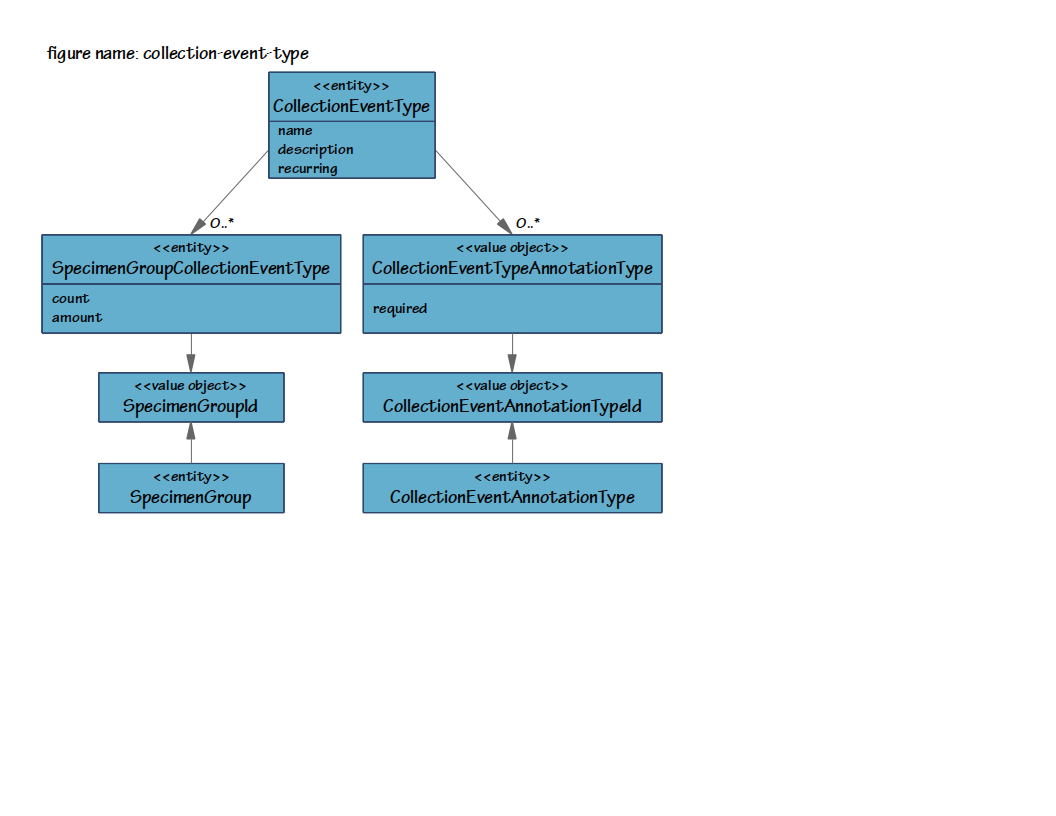
\includegraphics[trim={9mm 56mm 96mm 18mm}, clip,
    width=0.8\textwidth]{images/collection-event-type}
  \caption{Details for the CollectionEventType entity}
  \label{fig:collection-event-type}
\end{figure}

\subsection*{SpecimenGroupCollectionEventType}

\valobjtarget{SpecimenGroupCollectionEventType}s are used to define which types
of specimens (i.e. which \valobjlink{SpecimenGroup}s) need to be collected with
a type of collection event. A single specimen group can be used in multiple
collection event types.

The \compfont{count} specifies how many specimens are to be collected. The
\compfont{amount} is the amount of substance that is expected in each collected
specimen, or null if there is no default amount. The unit on the amount is
defined in the \entitylink{SpecimenGroup}.

\subsection*{CollectionEventAnnotationType}
Collection event annotations are defined using
\entitytarget{CollectionEventAnnotationType}. One or more of these can be
defined for the study. More details for this entity are given in Chapter
\ref{chap:study-annotations}.

\subsection*{CollectionEventTypeAnnotationType}
\valobjtarget{CollectionEventTypeAnnotationType} allows a single
\entitylink{CollectionEventAnnotationType} to be used in more than one
collection event. When the \compfont{required} field is set to \compfont{true},
the annotation value in \entitylink{CollectionEventAnnotation} is not allowed
to be empty. This class is a value object since it only serves to associate a
\valobjtarget{CollectionEventAnnotationTypeId} to a
\valobjtarget{CollectionEventTypeId}.

\section{ProcessingType Details}
\label{sec:processing-type}

A processing type has a name and an optional description. The name is a short
identifying name that is unique to the study, and the description can provide
additional details on the name. A processing type should have \compfont{enabled}
set to \compfont{true} when processing of the contained specimen types is taking
place. However, throughout the lifetime of the study, it may be decided to stop
a processing type in favour of another. In this case \compfont{enabled} is set to
\compfont{false}.

A processing type can be configured to process one or more collected specimens
using \valobjlink{SpecimenLinkType}. Individual specimen link types within the
processing type can also be configured to record one or more annotation using
\valobjlink{SpecimenLinkTypeAnnotationType}. Figure \ref{fig:processing-type}
provides more details for the processing type entity.

One or more processing types can be defined for a study. For specimen
processing to be allowed on a study, at least one processing type must be
defined.

\begin{figure}[H]
  \centering
  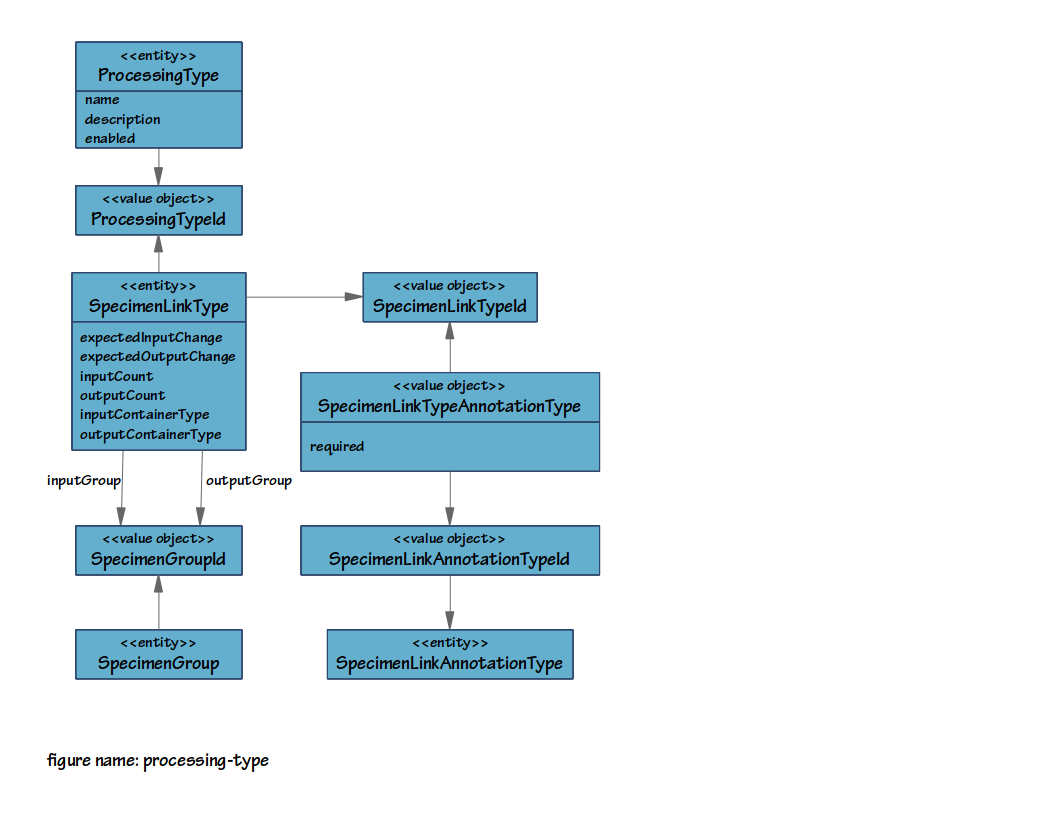
\includegraphics[trim={10mm 26mm 120mm 18mm}, clip,
    width=0.7\textwidth]{images/processing-type}
  \caption{Model for defining processing types.}
  \label{fig:processing-type}
\end{figure}

Processing of specimens is not allowed until at least one processing type is
defined for the study.

\subsection*{SpecimenLinkType}
\valobjtarget{SpecimenLinkType}s are assigned to
a processing type, and used to represent a regularly performed processing
procedure involving two \entitylink{Specimen}s: an input, which must be in a
specific \valobjlink{SpecimenGroup}, and an output, which must be in a specific
\valobjlink{SpecimenGroup}.

The \compfont{expectedInputChange} is the expected amount (decimal value) to be
removed from each input. The \compfont{expectedOutputChange} (also a decimal
value) is the expected amount to be added to each output. If the expected input
and output change values are not required, they can be assigned a zero value.
The counts in \compfont{inputCount} and \compfont{outputCount} are the number of
expected and resulting specimens, respectively, when the processing is carried
out. A value of zero for output count implies that the count is the same as the
input count. The specimen container type that holds the input specimens is
given in \compfont{inputContainerType}. The specimen container type that the
output specimens are stored into is given in \compfont{outputContainerType}. If
specifying the container types is not required for one or both of these fields,
they can be assigned a \compfont{null} value.

To avoid redundancy, each combination of \compfont{inputGroup} and
\compfont{outputGroup}) may exist only once per \entitylink{ProcessingType}.

\subsection*{SpecimenLinkTypeAnnotationType}

A \valobjtarget{SpecimenLinkTypeAnnotationType} is used to tie a specimen
link annotation type to a specimen link type.

\section {Study Aggregate Commands}
\subsection{Study Commands}
The commands handled by the study aggregate are listed below.

\subsection*{CreateStudyCommand}
Creates a new study. A study can be created at any time. If a study with the
given name already exists the command fails and throws a checked exception.

\begin{commandparmtable}

  name & String & A short descriptive name associated with the study. Usually
  an acronym.\\

  description & String & A more detailed name for the study. If an acronym is
  used for the study name, then the description should contain the words that
  make up the acronym.\\

\end{commandparmtable}

\subsection*{UpdateStudyCommand}

Update a study's name, description, or both. If a study with the
new name already exists the command fails and throws a checked exception.

\begin{commandparmtable}

  studyId & String & The study's unique identifier.\\

  name & String & The new name, or the original name if it's not being modified.\\

  description & String & The new description, or the original description if
  it's not being modified.\\

\end{commandparmtable}

\subsection*{EnableStudyCommand}

Enables a study. Once enabled the study is ready to collect and process
specimens from participants.

\begin{commandparmtable}

  studyId & String & The study's unique identifier.\\

\end{commandparmtable}

\subsection*{DisableStudyCommand}

Used to disable a study. A study may be disabled because no more specimen
collection and processing will be done on it, or because it requires
configuration changes. Once disabled specimen collection and processing cannot
be performed on this study.

\begin{commandparmtable}

  studyId & String & The study's unique identifier.\\

\end{commandparmtable}

\subsection{Specimen Group Commands}
\subsection*{CreateSpecimenGroupCommand}

Creates a specimen group on a study. If the study is not disabled the command
fails and throws a checked exception. If a specimen group already exists with
the given name the command fails and throws a checked exception.

\begin{commandparmtable}

  studyId & string & The study's unique identifier.\\

  name & string & A short descriptive name.\\

  description & string & Provides more details for the specimen group. Can be left empty.\\

  anatomicalSourceId & string & The ID corresponding to the anatomical source this group
  belongs to.\\

  preservationId & string & The ID corresponding to the preservation used by this
  specimen group.\\

  specimenTypeId & string & The ID corresponding to the specimen type.\\

\end{commandparmtable}

\subsection*{UpdateSpecimenGroupCommand}

Updates a specimen group on a study. If the study is not disabled the command
fails and throws a checked exception. If a specimen group already exists with
the new name the command fails and throws a checked exception.

\begin{commandparmtable}

  studyId & string & The study's unique identifier.\\

  name & string & The new name, or the original name if it's not being modified.\\

  description & string & The new description, or the original description if
  it's not being modified.\\

  anatomicalSourceId & string & The ID corresponding to the updated or original
  anatomical source.\\

  preservationId & string & The ID corresponding to the updated or original preservation.\\

  specimenTypeId & string & The ID corresponding to the updated or original specimen type.\\

\end{commandparmtable}

\subsection*{DeleteSpecimenGroupCommand}

Deletes a specimen group from the study. If the study is not disabled the
command fails and throws a checked exception.

\begin{commandparmtable}

  studyId & string & The study's unique identifier.\\

  specimenGroupId & string & The specimen group's unique identifier.\\

\end{commandparmtable}
% Local Variables:
% compile-command: "/usr/bin/rubber --pdf main"
% End:


\subsection{Collection Event Type Commands}

\subsection*{CreateCollectionEventType}
Creates a collection event type for a study. If the study is not disabled the
command fails and throws a checked exception. The command fails with a checked
exception if name already exists.
\begin{commandparmtable}

  studyId & string & The study's unique identifier.\\

  name & string & A short descriptive name.\\

  description & string & Provides more details. Can be left empty.\\

  recurring & boolean & Set to \compfont{true} if this collection event type
  occurs more than once for the duration of the study.\\

\end{commandparmtable}

\subsection*{UpdateCollectionEventType}
Updates one or more attributes of a collection event type. If a collection event with the
given name already exists the command fails and throws a checked exception.
\begin{commandparmtable}

  studyId & string & The study's unique identifier.\\

  collectionEventTypeId & string & The collection event type's unique identifier.\\

  name & string & The new name, or the original name if it's not being modified.\\

  description & string & The new description, or the original description if
  it's not being modified.\\

  recurring & boolean & The new value, or the original value if it's not being
  modified.\\

\end{commandparmtable}

\subsection*{DeleteCollectionEventType}
Deletes a collection event type.
\begin{commandparmtable}

  studyId & string & The study's unique identifier.\\

  collectionEventTypeId & string & The collection event type's unique identifier.\\

\end{commandparmtable}

\subsection*{AddSpecimenGroupToCollectionEventType}
Adds a specimen group to a collection event type.
\begin{commandparmtable}

  studyId & string & The study's unique identifier.\\

  collectionEventTypeId & string & The collection event type's unique identifier.\\

  specimenGroupId & string & The specimen group's unique identifier.\\

\end{commandparmtable}

\subsection*{RemoveSpecimenGroupFromCollectionEventType}
Removes a specimen group from a collection event type.
\begin{commandparmtable}

  studyId & string & The study's unique identifier.\\

  collectionEventTypeId & string & The collection event type's unique identifier.\\

  specimenGroupId & string & The specimen group's unique identifier.\\

\end{commandparmtable}

\subsection*{AddAnnotationToCollectionEventType}
Adds an annotation type to a collection event type.

\begin{commandparmtable}

  studyId & string & The study's unique identifier.\\

  collectionEventTypeId & string & The collection event type's unique identifier.\\

  collectionEventAnnotationTypeId & string & The annotation type's unique identifier.\\

\end{commandparmtable}

\subsection*{RemoveAnnotationFromCollectionEventType}
Removes an annotation type from a collection event type.

\begin{commandparmtable}

  studyId & string & The study's unique identifier.\\

  collectionEventTypeId & string & The collection event type's unique identifier.\\

  collectionEventAnnotationTypeId & string & The annotation type's unique identifier.\\

\end{commandparmtable}
% Local Variables:
% compile-command: "/usr/bin/rubber --pdf main"
% End:


\subsection{Processing Type Commands}

\subsection*{CreateProcessingType}
Creates a processing type for a study. If the study is not disabled the command
fails and throws a checked exception. The command fails with a checked
exception if name already exists.

\begin{commandparmtable}

  studyId & string & The study's unique identifier.\\

  name & string & A short descriptive name.\\

  description & string & Provides more details. Can be left empty.\\

  enabled & boolean & Set to \texttt{true} when this processing type is still
  in use.\\

\end{commandparmtable}

\subsection*{UpdateProcessingType}
Updates one or more attributes of a processing type. If a processing with the
given name already exists the command fails and throws a checked exception.

\begin{commandparmtable}

  studyId & string & The study's unique identifier.\\

  processingTypeId & string & The processing type's unique identifier.\\

  name & string & The new name, or the original name if it's not being modified.\\

  description & string & The new description, or the original description if
  it's not being modified.\\

  enabled & boolean & The new value, or the original value if it's not being
  modified.\\

\end{commandparmtable}

\subsection*{DeleteProcessingType}
Deletes a processing type.

\begin{commandparmtable}

  studyId & string & The study's unique identifier.\\

  processingTypeId & string & The processing type's unique identifier.\\

\end{commandparmtable}

\subsection*{EnableProcessingType}
Used to enable a processing type that was previously disabled.

\begin{commandparmtable}

  studyId & string & The study's unique identifier.\\

  processingTypeId & string & The processing type's unique identifier.\\

\end{commandparmtable}

\subsection*{DisableProcessingType}
Used to disable a processing type that was previously enabled.

\begin{commandparmtable}

  studyId & string & The study's unique identifier.\\

  processingTypeId & string & The processing type's unique identifier.\\

\end{commandparmtable}

\subsection*{AddSpecimenLinkType}

\begin{commandparmtable}

  studyId & string & The study's unique identifier.\\

  processingTypeId & string & The processing type's unique identifier.\\

  expectedInputChange & decimal & Amount to be removed from input. Use a value
  of zero if amount change tracking is not required.\\

  expectedOutputChange & decimal & Amount to be added to each output. Use a value
  of zero if amount change tracking is not required.\\

  inputCount & integer & The number of expected specimens.\\

  outputCount & integer & The number of resulting specimens after processing. A
  value of zero implies that the output count is the same as the input count.\\

  inputContainerType & \entitylink{SpecimenContainer} & The specimen container type
  that holds the input specimens.\\

  outputContainerType & \entitylink{SpecimenContainer} & The specimen container type
  that holds the output specimens.\\

\end{commandparmtable}

\subsection*{UpdateSpecimenLinkType}

\begin{commandparmtable}

  studyId & string & The study's unique identifier.\\

  processingTypeId & string & The processing type's unique identifier.\\

  specimenLinkTypeId & string & The specimen link type's unique identifier.\\

  expectedInputChange & decimal & The new or original input change amount.\\

  expectedOutputChange & decimal & The new or original output change amount.\\

  inputCount & integer & The new or original number expected specimens.\\

  outputCount & integer & The new or original number of resulting specimens.\\

  inputContainerType & \entitylink{SpecimenContainer} & The new or original
  input specimen container type.\\

  outputContainerType & \entitylink{SpecimenContainer} & The new or original
  output specimen container type.\\

\end{commandparmtable}

\subsection*{RemoveSpecimenLinkType}

\begin{commandparmtable}

  studyId & string & The study's unique identifier.\\

  processingTypeId & string & The processing type's unique identifier.\\

  specimenLinkTypeId & string & The specimen link type's unique identifier.\\

\end{commandparmtable}

\subsection*{AddInputSpecimenGroupToSpecimenLinkType}

\begin{commandparmtable}

  studyId & string & The study's unique identifier.\\

  processingTypeId & string & The processing type's unique identifier.\\

  specimenLinkTypeId & string & The specimen link type's unique identifier.\\

  specimenGroupId & string & The specimen group's unique identifier.\\

\end{commandparmtable}

\subsection*{RemoveInputSpecimenGroupFromSpecimenLinkType}

\begin{commandparmtable}

  studyId & string & The study's unique identifier.\\

  processingTypeId & string & The processing type's unique identifier.\\

  specimenLinkTypeId & string & The specimen link type's unique identifier.\\

  specimenGroupId & string & The specimen group's unique identifier.\\

\end{commandparmtable}

\subsection*{AddOutputSpecimenGroupToSpecimenLinkType}

\begin{commandparmtable}

  studyId & string & The study's unique identifier.\\

  processingTypeId & string & The processing type's unique identifier.\\

  specimenLinkTypeId & string & The specimen link type's unique identifier.\\

  specimenGroupId & string & The specimen group's unique identifier.\\

\end{commandparmtable}

\subsection*{RemoveOutputSpecimenGroupFromSpecimenLinkType}

\begin{commandparmtable}

  studyId & string & The study's unique identifier.\\

  processingTypeId & string & The processing type's unique identifier.\\

  specimenLinkTypeId & string & The specimen link type's unique identifier.\\

  specimenGroupId & string & The specimen group's unique identifier.\\

\end{commandparmtable}

\subsection*{AddAnnotationToSpecimenLinkType}

\begin{commandparmtable}

  studyId & string & The study's unique identifier.\\

  processingTypeId & string & The processing type's unique identifier.\\

  specimenLinkTypeId & string & The specimen link type's unique identifier.\\

  specimenLinkAnnotationTypeId & string & The specimen link annotation types's
  unique identifier.\\

  required & boolean & Use \texttt{true} when this annotation type is required
  and cannot be left empty.\\

\end{commandparmtable}

\subsection*{RemoveAnnotationFromSpecimenLinkType}

\begin{commandparmtable}

  studyId & string & The study's unique identifier.\\

  processingTypeId & string & The processing type's unique identifier.\\

  specimenLinkTypeId & string & The specimen link type's unique identifier.\\

  specimenLinkAnnotationTypeId & string & The specimen link annotation types's
  unique identifier.\\

\end{commandparmtable}


% Local Variables:
% compile-command: "/usr/bin/rubber --pdf main"
% End:


\chapter{Specimen Collection}

The \entitylink{Participant} aggregate is used to record specimens collected
from study participants.

\begin{figure}[H]
  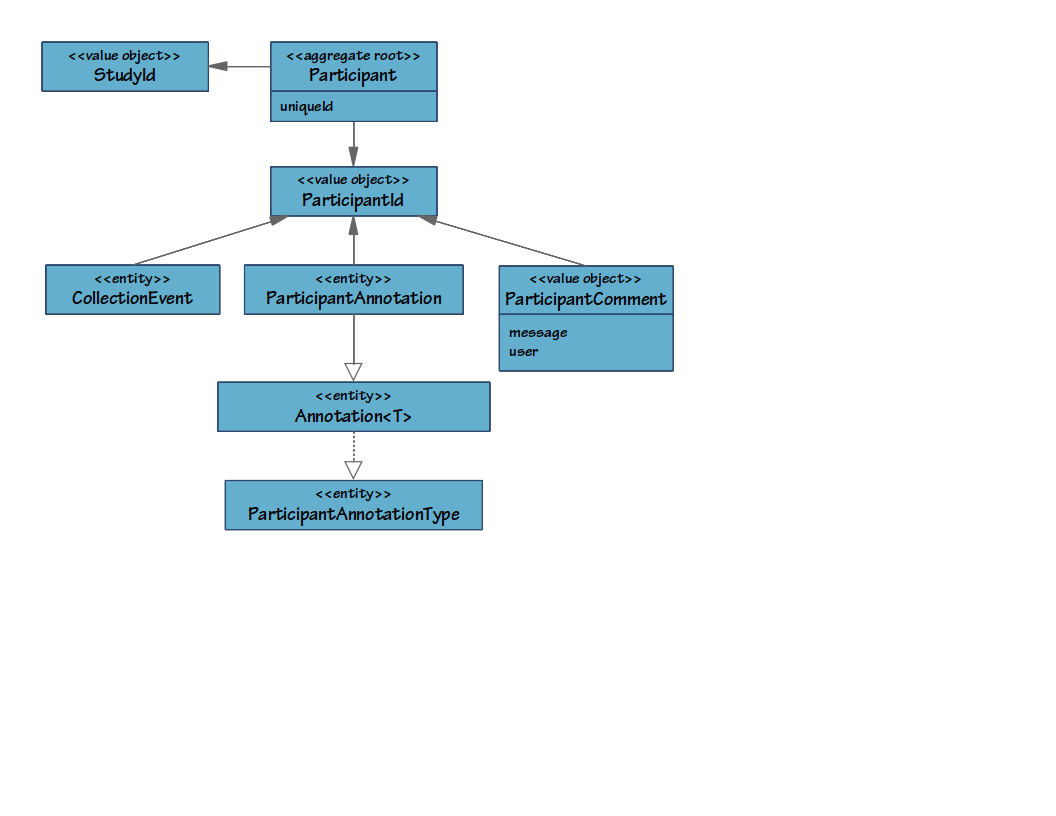
\includegraphics[trim={10mm 75mm 102mm 10mm}, clip,
    width=0.75\textwidth]{images/participant-aggregate}
  \caption{Participant aggregate}
  \label{fig:participant-aggregate}
\end{figure}

\begin{figure}[H]
  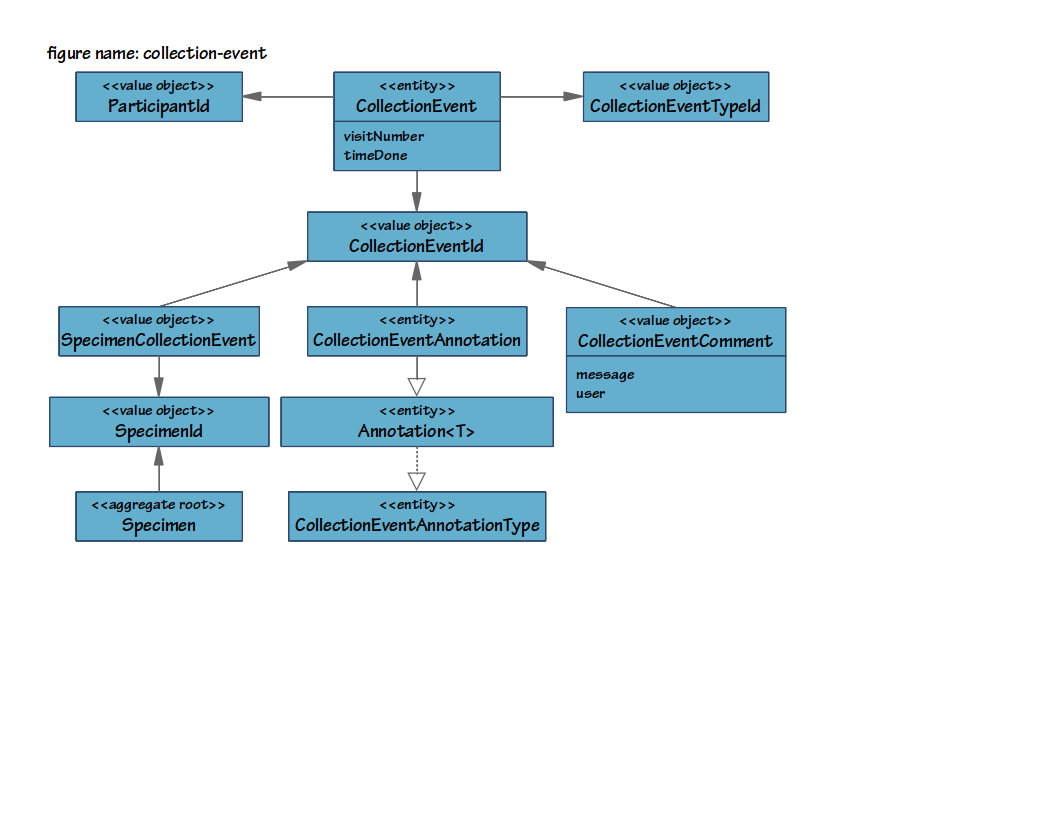
\includegraphics[trim={10mm 66mm 75mm 10mm}, clip,
    width=0.85\textwidth]{images/collection-event}
  \caption{CollectionEvent entity}
  \label{fig:collection-event}
\end{figure}

\chapter{Specimen Processing and Storage}
\label{chap:specimen-processing}

When a specimen is processed portions of it are used to create aliquots or
derivative specimens. Figure \ref{fig:specimen-aggregate} shows the model to
record the processing information.

\begin{figure}[H]
  \centering
  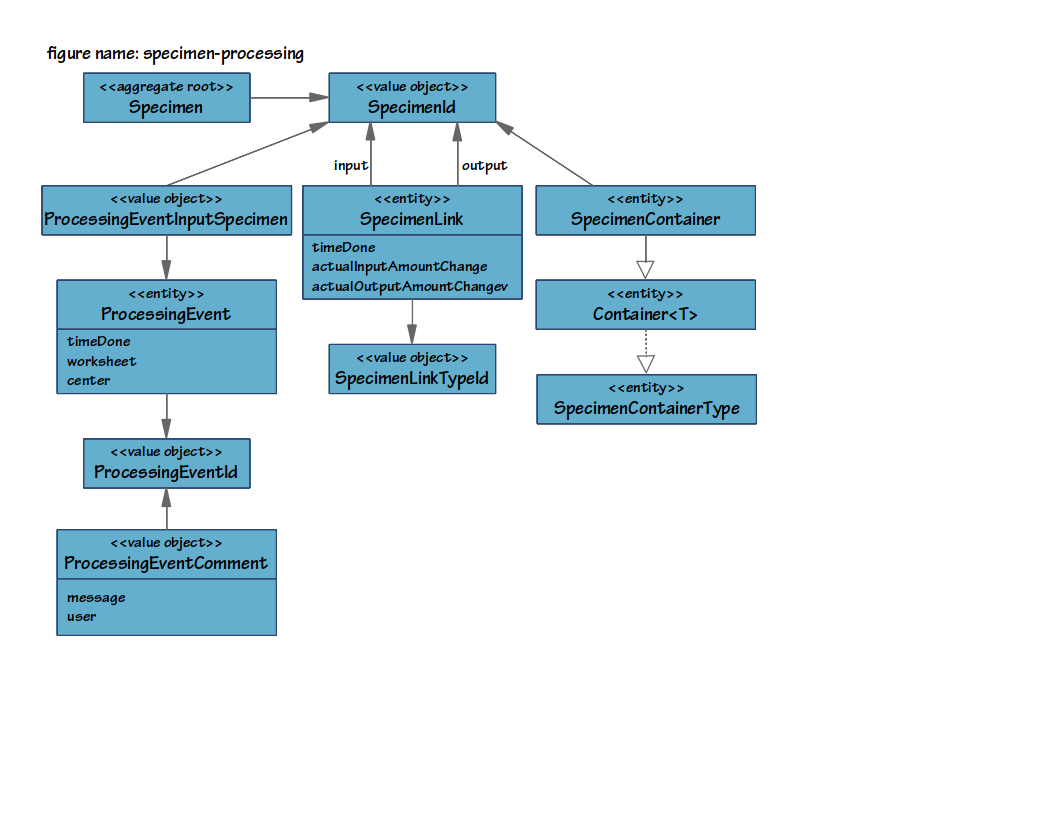
\includegraphics[trim={10mm 42mm 78mm 18mm}, clip,
    width=0.75\textwidth]{images/specimen-processing}
  \caption{Specimen Processing Model}
  \label{fig:specimen-processing}
\end{figure}

\subsection*{ProcessingEvent}
The \entitytarget{ProcessingEvent} entity records information about a group of
specimens that were processed at the same time. The processing event has the
following attributes: \compfont{timeDone} the time stamp for when the
processing took place; \compfont{worksheet} a unique identifier associated with
the processing event used to cross reference to other systems;
\compfont{center} the processing center where the processing is taking place.

\subsection*{ProcessingEventInputSpecimen}
It is possible that a single specimen be processed multiple
times. \entitytarget{ProcessingEventInputSpecimen} is used to record this.

\subsection*{SpecimenLink}
\entitytarget{SpecimenLink} is a record of the specimens and amounts involved
in a \entitylink{SpecimenLinkType}. This entity provides more detailed
information about the parentage of a specimen, i.e. the \compfont{input-output}
pair could be considered a parent-child relationship. This is opposed to
collection events, which provide much more general heritage information. So,
special care must be taken to ensure that \entitylink{SpecimenCollectionEvent}
and \entitylink{SpecimenLink} entities are consistent. The \compfont{output}
must be in all the same collection events as the \compfont{input}, but if two
specimens are in the same collection event they do \emph{not} need to be
associated (directly or transitively) through a \entitylink{SpecimenLink}. Also
note that the \compfont{input} does \emph{not} need to be in the same
collection event(s) as the \compfont{output}.

\subsection*{SpecimenContainer}
The container that holds this specimen. Specimen containers are containers that
only hold specimens. More information for containers is given in Chapter
\ref{containers}.

\subsection*{ProcessingEventComment}
A \entitytarget{ProcessingEventComment} contains a textual message and the
user that added the comment. The date and time the comment was made is recorded
as meta data. A processing event can have one or more comments.

% Local Variables:
% compile-command: "/usr/bin/rubber --pdf main"
% End:

\chapter{Annotations}
\label{chap:annotations}

Annotations allow a study to collect custom named and defined pieces of data
for participants, collection events, and specimen processing. Figure
\ref{fig:annotation-example} shows the annotation entities related to
participant annotations. The annotations for collection event and specimen
processing are similar. Annotations are optional and are not required to be
defined for a study.

\begin{figure}[H]
  \centering
  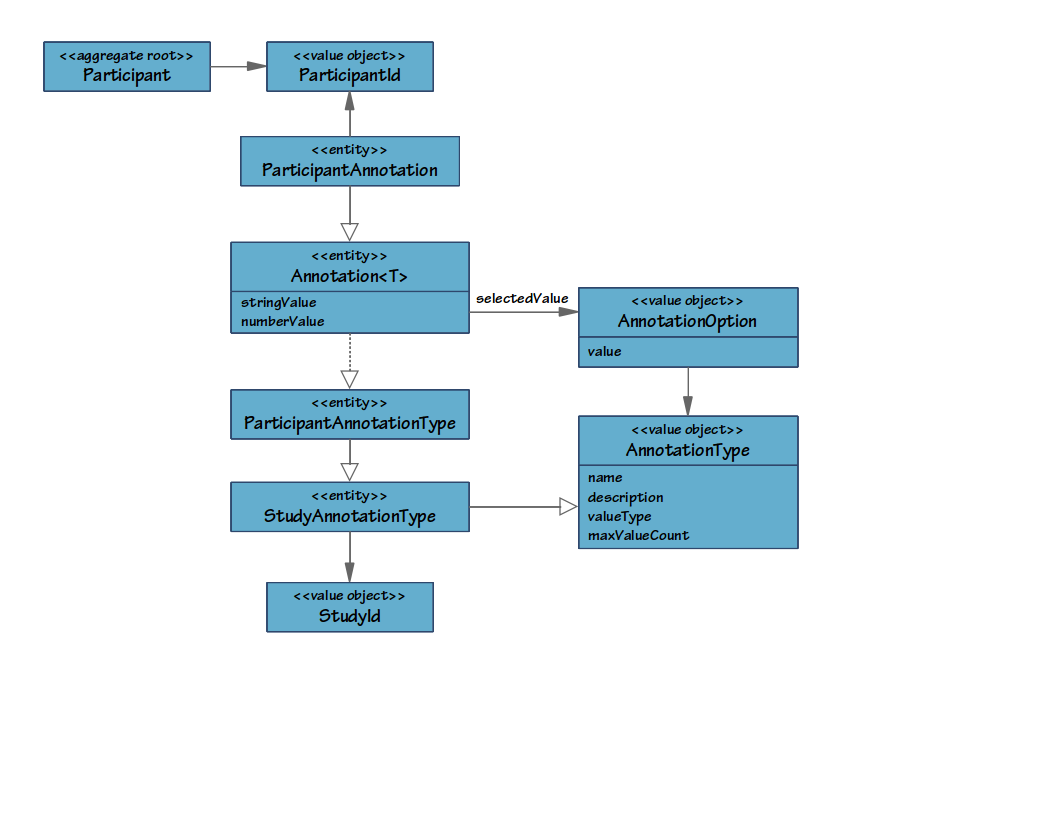
\includegraphics[trim={10mm 45mm 68mm 10mm}, clip,
    width=0.8\textwidth]{images/annotation-example}
  \caption{Annotations example}
  \label{fig:annotation-example}
\end{figure}

The \entitylink{ParticipantAnnotation} is a derived class of the generic class
\entitytarget{Annotation}. Possible annotations for a study are defined using
\entitylink{ParticipantAnnotationType} which is a derived class for
\entitylink{StudyAnnotationType} which itself is a derived class of
\entitytarget{AnnotationType}.

An annotation type has a short identifying name that is unique to the study. A
description can also be defined but is optional. The following table shows the
possible values for \compfont{valueType}. The value type specifies what the
annotation stores.

\begin{table}[H]
\renewcommand{\arraystretch}{1.1}
\begin{tabularx}{\textwidth}{@{\hspace{6pt}} >{\ttfamily}l X }
  \sffamily{\textbf{Value Type}} & \sffamily{\textbf{What is stored}}\\
  \hline

  String & an alphanumeric string.\\
  Number & a number, either integer or decimal.\\
  Date & date string, usually of the form \emph{YYYY-MM-DD HH:MM}.\\
  Select & a value selected from a predefined list.\\

\end{tabularx}
\end{table}

When \compfont{valueType} is assigned to be of type \compfont{Select},
\compfont{maxValueCount} is the number of of items that can be selected from the
predefined list. If only one value is allowed, then \compfont{maxValueCount} has
a value of 1. If an unlimited number of values are allowed then,
\compfont{maxValueCount} has a value of 0.

One or more \entitylink{AnnotationOption}s are used to create the predefined
list of select options.

Of the fields \compfont{stringValue}, \compfont{numberValue}, or
\compfont{selectedValue} in \entitytarget{Annotation}, only a single one is
used to store the annotation value. The remaining fields are
\compfont{null}. The field that is used is referred to as the \emph{Value
  Field}. The Value Field used depends on the value
\compfont{AnnotationType.valueType}.

\begin{table}[!htbp]
\renewcommand{\arraystretch}{1.1}
\begin{tabularx}{\textwidth}{@{\hspace{6pt}} >{\ttfamily}l l}
  \sffamily{\textbf{ValueType}} & \sffamily{\textbf{Value field}}\\
  \hline
  String & \compfont{stringValue}\\
  Number & \compfont{numberValue}\\
  Date & \compfont{numberValue} and stored as the number of seconds\\
  Select & \compfont{selectedValue}\\

\end{tabularx}
\end{table}


%----------------------------------------------------------------------------------------
% Bibliography
%----------------------------------------------------------------------------------------

\chapter*{Bibliography}
\addcontentsline{toc}{chapter}{Bibliography}
\printbibliography[heading=bibempty]

\end{document}

% Local Variables:
% compile-command: "/usr/bin/rubber --pdf main"
% End:

